\subsubsection{Presentation}
Ensemble learning models combine results of multiple models to improve overall performance.\\
There are many different techniques in which to apply this concept, we will be using a RandomForestClassifier, which falls under the bagging ensemble techniques.\\
Bagging is simply the idea of splitting the data into subsets and training a model on each subset, then combining the results to achieve a more generalized result, a RandomForestClassifier uses Decision Trees as the internal models.

\subsubsection{Defining Parameters}
The data for training and validating is already defined by the Data Preparation step (80\% train, 20\% validation).\\
Representative parameters for the model are \emph{n\_estimators}, \emph{max\_features}, and \emph{max\_depth}.
\begin{itemize}
    \item \underline{n\_estimators}: The number of internal models used in the ensemble.
    \item \underline{max\_features}: The maximum number of features allowed for the split in each decision tree.
    \item \underline{max\_depth}: The maximum depth of each tree in the ensemble.
\end{itemize}
We trained an ensemble using a GridSearch over a few different values of these parameters to see if we can achieve a higher accuracy than the defaults.\\
We achieved 96.4\% accuracy with the parameters set to {'bootstrap': True, 'max\_depth': 50, 'max\_features': 10, 'n\_estimators': 200}, only a slightly (0.2\%) higher accuracy score than default parameters.
Tuning this model proved difficult as it was overfitting the data very fast, as we can see from this complexity curves over different values of \emph{n\_estimators} and \emph{max\_depth}. \\
\begin{center}
    \captionsetup{type=figure}
    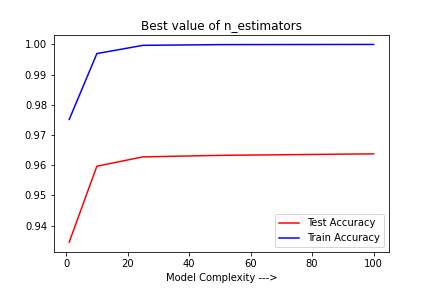
\includegraphics[width=250px]{RF_complexity_estimators.png}
    \captionof{figure}{Complexity Curve: \emph{n\_estimators} value for RFC}
\end{center}

\begin{center}
    \captionsetup{type=figure}
    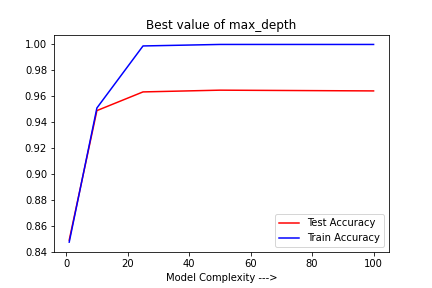
\includegraphics[width=250px]{RF_complexity_depth.png}
    \captionof{figure}{Complexity Curve: \emph{max\_depth} value for RFC}
\end{center}
\subsubsection{Model Evaluation}
We plotted the learning curve for the model using default params, over the training data split (around 90k rows).
\begin{center}
    \captionsetup{type=figure}
    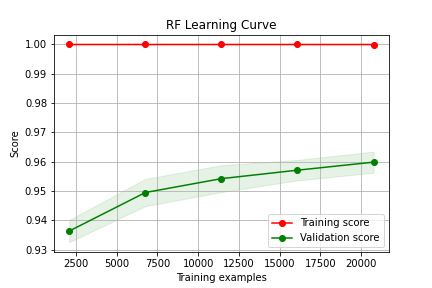
\includegraphics[width=250px]{learning_curve_RF_small.png}
    \captionof{figure}{Learning Curve for RFC over large dataset}
\end{center}
It shows a very high bias and an almost immediate overfitting, so as an experiment we plotted the learning curve over a smaller data split (in this case our validation split, about 30k rows) it showed how quickly the model overfits the training data.
\begin{center}
    \captionsetup{type=figure}
    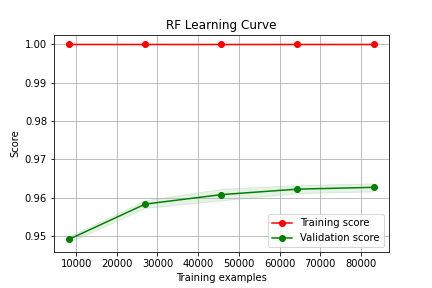
\includegraphics[width=250px]{learning_curve_RF_big.png}
    \captionof{figure}{Learning Curve for RFC over small dataset}
\end{center}